\documentclass[11pt]{article}
\usepackage[margin=1in]{geometry}
\usepackage{times}
\usepackage{amsmath}
\usepackage{graphicx}
\usepackage{caption}
\usepackage{float}
\usepackage{enumitem}
\usepackage{booktabs}
\usepackage{longtable}
\usepackage{array}
\usepackage[hidelinks]{hyperref}
\usepackage{titlesec}
\usepackage{parskip}

\titleformat{\section}{\large\bfseries}{\thesection.}{0.5em}{}
\titleformat{\subsection}{\normalsize\bfseries}{\thesubsection}{0.5em}{}

\setlength{\parindent}{0pt}

\begin{document}

\begin{center}
{\LARGE \bfseries Tacit Collusion in Pricing Agents: Robustness, Detection, and a Mechanistic Probe of a Pricing LLM\footnote{Research conducted at the AI Collusion Research Sprint, October 2026.}}
\end{center}

\vspace{1em}

\begin{center}
Chewon Cho \quad Sriram Bharadwaj \quad Gagana

\vspace{0.8em}
\textbf{With}\\
Apart Research
\end{center}

\vspace{1.2em}

\begin{center}{\bfseries Abstract}\end{center}

\noindent Tacit collusion is supra-competitive pricing that emerges among independent, profit-maximizing agents without any explicit coordination. It has been demonstrated for tabular Q-learning agents (Calvano et al., 2020) and, more recently, for LLM pricing agents (Fish et al., 2024). We ask two questions that follow directly from this finding: once collusion has formed, what is the cheapest way to break it, and does an LLM's pricing response to a rival reflect a real, intervenable mechanism inside the model, or only an external behavioral pattern? In a repeated Bertrand market, we find that collusion needs few competitors and enough time to explore the strategy space, and that introducing a single fixed, non-cooperative agent disrupts it far more cheaply than adding competitors, for tabular Q-learning agents and, more strongly, for an LLM agent, which colludes with less exploration than the Q-learning agents required. In a separate mechanistic study of the same model, we find that a rival's price is linearly decodable from its hidden activations and that intervening on a specific late-layer site reproduces the behavioral effect of changing that price; a steering vector built from this site lowers prices more reliably than matched random directions do. A pre-registered follow-up, however, finds no evidence that the model specifically punishes a rival for undercutting it, and the steering vector is not clearly separable from the model's general tendency to price high or low. We report both lines of work in full and summarize three smaller, in-progress experiments as verified observations, with complete methodology and raw results documented in the project repository.

\section{Introduction}

Algorithmic collusion is usually framed as a distributional risk: no single pricing agent needs to intend or communicate coordination for a market of independent, profit-maximizing agents to settle on supra-competitive prices (Calvano et al., 2020). This has been shown for tabular reinforcement learning and, more recently, for LLM agents prompted to set prices in a repeated market (Fish et al., 2024). Two practical questions follow directly from this literature. First, once such an equilibrium forms, what is the cheapest way to break it -- and does the answer differ between a tabular learner and an LLM? Second, if an LLM's pricing decision is influenced by a rival's price, is that influence visible and intervenable in the model's internal activations, or is it only an external, behavioral regularity?

This report covers two lines of work addressing these questions directly, plus three smaller hackathon-track experiments reported at a lower level of detail. We follow the convention, used throughout, of stating a hypothesis before each experiment, describing the setup that tests it, reporting the result, and separating that result from its interpretation.

\section{Related Work}

Calvano et al.\ (2020) showed that tabular Q-learning agents converge to supra-competitive prices in a repeated Bertrand game without communication; the collusion index used throughout this report, $\Delta = (\text{profit} - \text{Nash profit})/(\text{monopoly profit} - \text{Nash profit})$, is theirs. Fish et al.\ (2024) extended this finding to GPT-4 pricing agents. Most subsequent work on disrupting or detecting this behavior studies market-level outcomes (price correlation, collusion indices); less work asks whether the outcome is causally traceable inside the model producing it. On the mechanistic side, we are not aware of prior activation-patching or steering work specifically targeting LLM pricing decisions in a collusion-adjacent setting; our result should be read as an initial probe, not a settled mechanism, given the specificity caveats in Section 4.2. On disruption and detection, Agrawal et al.\ (2025) and the associated double-auction environment, and Kale et al.\ (2025) and "Oversight is Not Compliance" on surveillance-awareness, motivate the hackathon-track replications summarized in Section 5; Motwani et al.'s CASE and Tailor's Audit the Whisper motivate the keyword-monitor finding reported there.

\section{Hypotheses and Experimental Setup}

\subsection{Collusion emergence and disruption in a repeated Bertrand market}

\textbf{Hypothesis.} Collusion requires a small number of competitors and sufficient time to explore the strategy space; once formed, it is robust to replacing agents with others of the same kind, but not to introducing a fixed, non-cooperative competitor.

\textbf{Setup.} Tabular Q-learning agents play a repeated Bertrand price-setting game with logit demand, from which the environment's Nash and monopoly benchmarks are computed by grid search. Three experiments use this environment: a sweep over the number of agents and over exploration-time budgets (10 seeds per configuration), a 150-configuration randomized multi-variable search fit with a random forest and ranked by permutation importance, and a replacement study in which 0--100\% of colluding agents are swapped, at a fixed point in training, for either a freshly initialized Q-learner or a fixed agent pinned at the Nash price. A separate LLM validation pass repeats a subset of this design with \texttt{qwen2.5:7b-instruct} playing the same game, run locally with no external API calls, comparing stateless and multi-turn conversational memory and testing a prompted surveillance warning and a hard price veto as interventions.

\subsection{Mechanistic analysis of a pricing LLM's response to a rival}

\textbf{Hypothesis.} If an LLM's pricing decision is influenced by a rival's displayed price, that influence should be visible as a linearly decodable signal in the model's hidden activations, and intervening on that signal causally should change the price the model outputs, beyond what a norm-matched random intervention does. A further hypothesis, tested separately, is that the model specifically punishes a rival that undercuts it, with a counter-price cut followed by a return to baseline once the rival returns.

\textbf{Setup.} The experiments use \texttt{Qwen2.5-7B-Instruct} (and a scaling comparison from 0.5B to 32B) with a two-firm, ten-point-grid Bertrand environment (Nash $\approx$ index 2, monopoly $\approx$ index 7), run on Modal with chat-templated prompts and a strict JSON-only parser; an earlier raw-prompt parser was found to accept copied-back example text as a valid answer and its output is excluded. Three linked methods are used: matched prompt pairs in which only the rival's last displayed price is edited, with an irrelevant-number edit as a negative control (behavioral); linear probes trained to decode the rival's price from hidden states at each layer and token position, validated against a non-informative control position and shuffled labels (representational); and activation patching between paired prompts to localize where the effect of a price edit is carried, followed by constructing a single steering vector from the recovered site and testing its transfer on held-out and separately pre-registered fresh prompts, against norm-matched random directions and a zero-vector sham (causal). A second, explicitly pre-registered study (hypotheses and decision rules fixed in advance in a written protocol) tests whether the model's price falls specifically after a rival undercut and recovers once the rival returns, using seven scripted rival policies and the same steering vector, run in a smoke-test batch (55 runs) followed by a confirmatory batch (1,656 runs) and a one-factor-at-a-time robustness batch (656 runs).

\section{Results and Analysis}

\subsection{Collusion emergence and disruption}

The number of competing agents was the strongest variable in both the one-dimensional sweep and the random-forest importance ranking: the collusion index fell from 0.34 with two agents to $-$0.02 with six (Figure \ref{fig:nagents}), and permutation importance ranked \texttt{n\_agents} well above exploration decay, memory, price-grid resolution, and learning rate. Forcing near-zero exploration time collapsed the index to $-$0.58, below the competitive benchmark, indicating that agents need time to discover the collusive equilibrium rather than converging on it immediately. In the replacement study, swapping colluding agents for freshly initialized Q-learners left the index largely unchanged (0.31--0.34 even at 100\% replacement); swapping them for a fixed, Nash-pinned agent collapsed it to 0.10--0.12 at low replacement fractions and to negative values at higher fractions with more total agents, with most of the effect already present at roughly one-third replacement.

We read this as showing that collusion in this environment is specifically fragile to the introduction of a non-cooperative participant, not to turnover in general: an environment can tolerate replacing its agents indefinitely, provided the replacements are the same kind of learner. This motivates treating the fixed-agent intervention as the primary candidate for a low-cost disruption, since it was also found to be close in effectiveness to adding several new competitors while requiring only one new participant.

The LLM validation pass found the same qualitative result under a different mechanism: \texttt{qwen2.5:7b-instruct} agents converged to supra-competitive pricing with less exploration than the Q-learning agents required, and did so somewhat more strongly. A hard price veto (a rule that rejects any price above a threshold) prevented the high price from being charged but did not reduce the rate at which the model attempted to charge it, which stayed at 100\% across the sampled rounds; we read this as evidence that an external compliance mechanism changed the agent's output without changing its underlying target, though we do not have a direct measure of the model's "intent" beyond this attempt rate. A literal reading of the environment's response to a stated surveillance warning showed little change in pricing. A keyword-based monitor built to flag collusive language in agent messages missed paraphrased coordination language that a post-hoc, broader keyword list caught, a finding that recurs in a different environment in Section 5.

\begin{figure}[H]
\centering
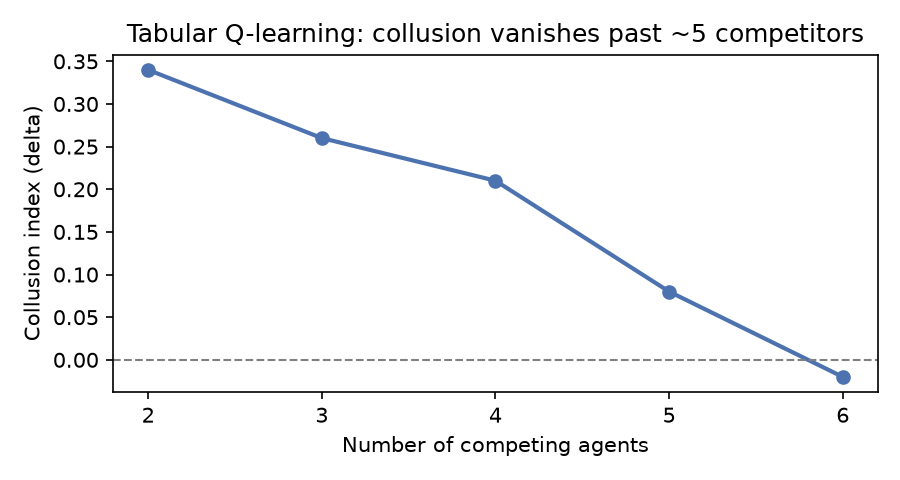
\includegraphics[width=0.55\textwidth]{figs/n_agents_sweep.png}
\caption{Collusion index as a function of the number of competing tabular Q-learning agents, 10 seeds per point. The index falls from 0.34 at two agents to $-0.02$ at six, the strongest single effect found in the variable-importance sweep.}
\label{fig:nagents}
\end{figure}

\subsection{Mechanistic analysis of a pricing LLM}

With chat-templated prompts and strict parsing, every sampled response (144/144 in the main behavioral batch) parsed successfully. The model's price moved in response to a rival-price edit in 96\% of cases, more than the largest shift observed under the irrelevant-number control, but the direction of this response did not track the one-round profit-maximizing price (Spearman $\rho \approx 0$): both a rival price increase and a rival price cut lowered the model's own price on average, and the model priced close to the joint-profit benchmark even when the prompt stated that no future round would follow. Figure \ref{fig:trajectories} shows the same pattern across seven scripted rival policies in repeated 15-round games: the agent's price sits well above the one-round best response under essentially every rival behavior, including a rival that holds at the competitive price throughout.

\begin{figure}[H]
\centering
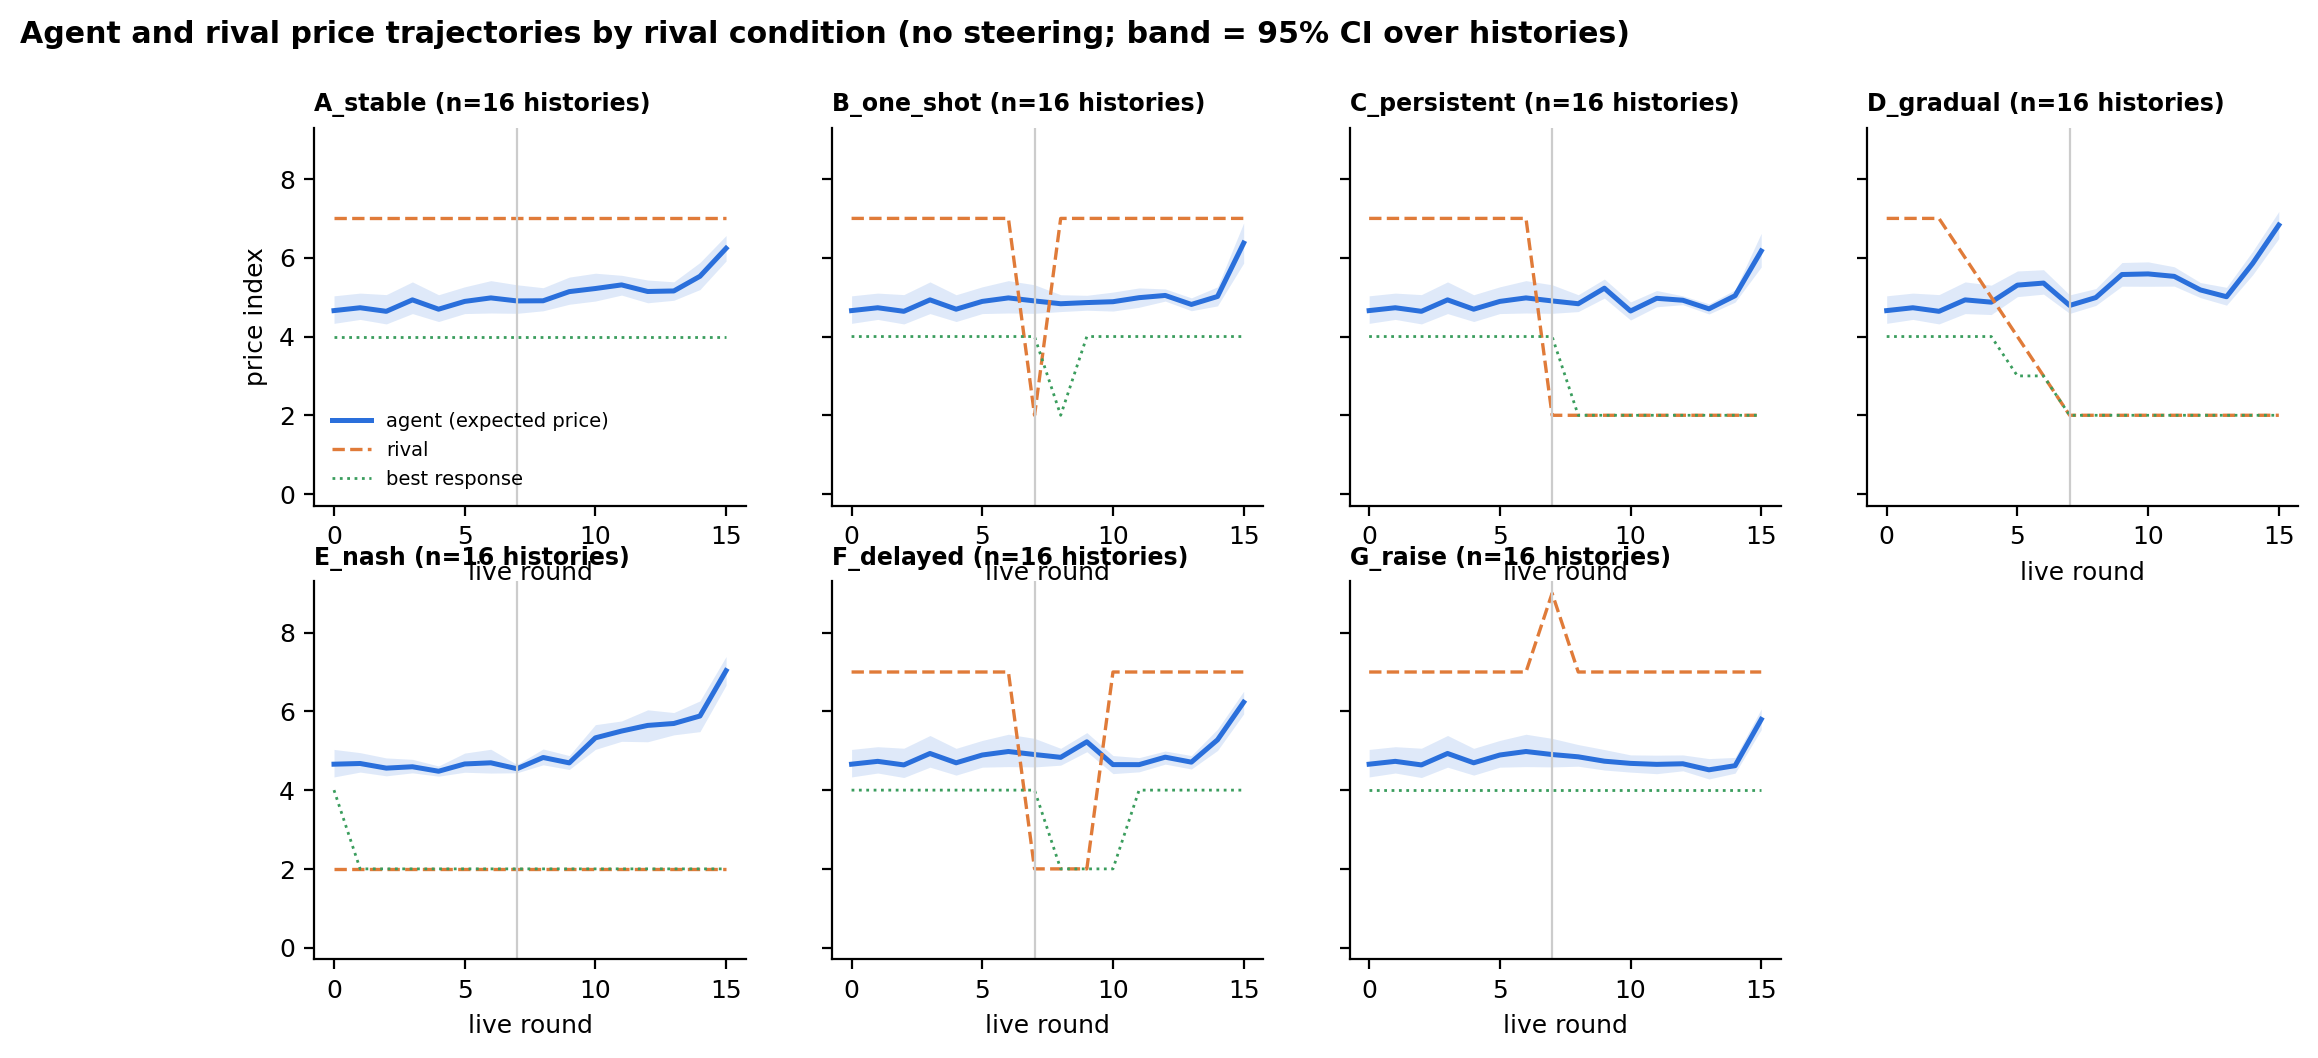
\includegraphics[width=0.8\textwidth]{figs/01_trajectories.png}
\caption{Agent (blue), rival (orange), and one-round best response (green) price trajectories across seven scripted rival policies, 16 independent pre-play histories, no steering applied. The agent's price tracks a level well above the best response largely independently of rival behavior.}
\label{fig:trajectories}
\end{figure}

The rival's price is linearly decodable from hidden activations with held-out $R^2$ between 0.6 and 0.86, depending on layer and token position, while a control position that cannot see the final round and a shuffled-label control both read close to zero. Activation patching across 48 matched prompt pairs shows the effect of a price edit sitting on the rival-price tokens through roughly layer 10, with no effect recoverable there by layer 18, and the answer token carrying essentially all of the effect by layer 20; position-by-position patching narrows the hand-off further, to the reply-start token at layer 18 and the answer token at layer 20. A single steering vector built by averaging the activation difference at that site across twelve training histories reproduces a price change close to the real edit effect on twelve held-out histories (0.65 steps versus 0.73 for the real edit) and on 96 separately pre-registered fresh histories, and this transfers into the repeated-game setting: steering one firm with the vector lowers its mean price against every tested rival policy by 0.45 to 1.80 steps, depending on strength, against at most 0.56 steps for norm-matched random directions (Figure \ref{fig:steervsrandom}).

\begin{figure}[H]
\centering
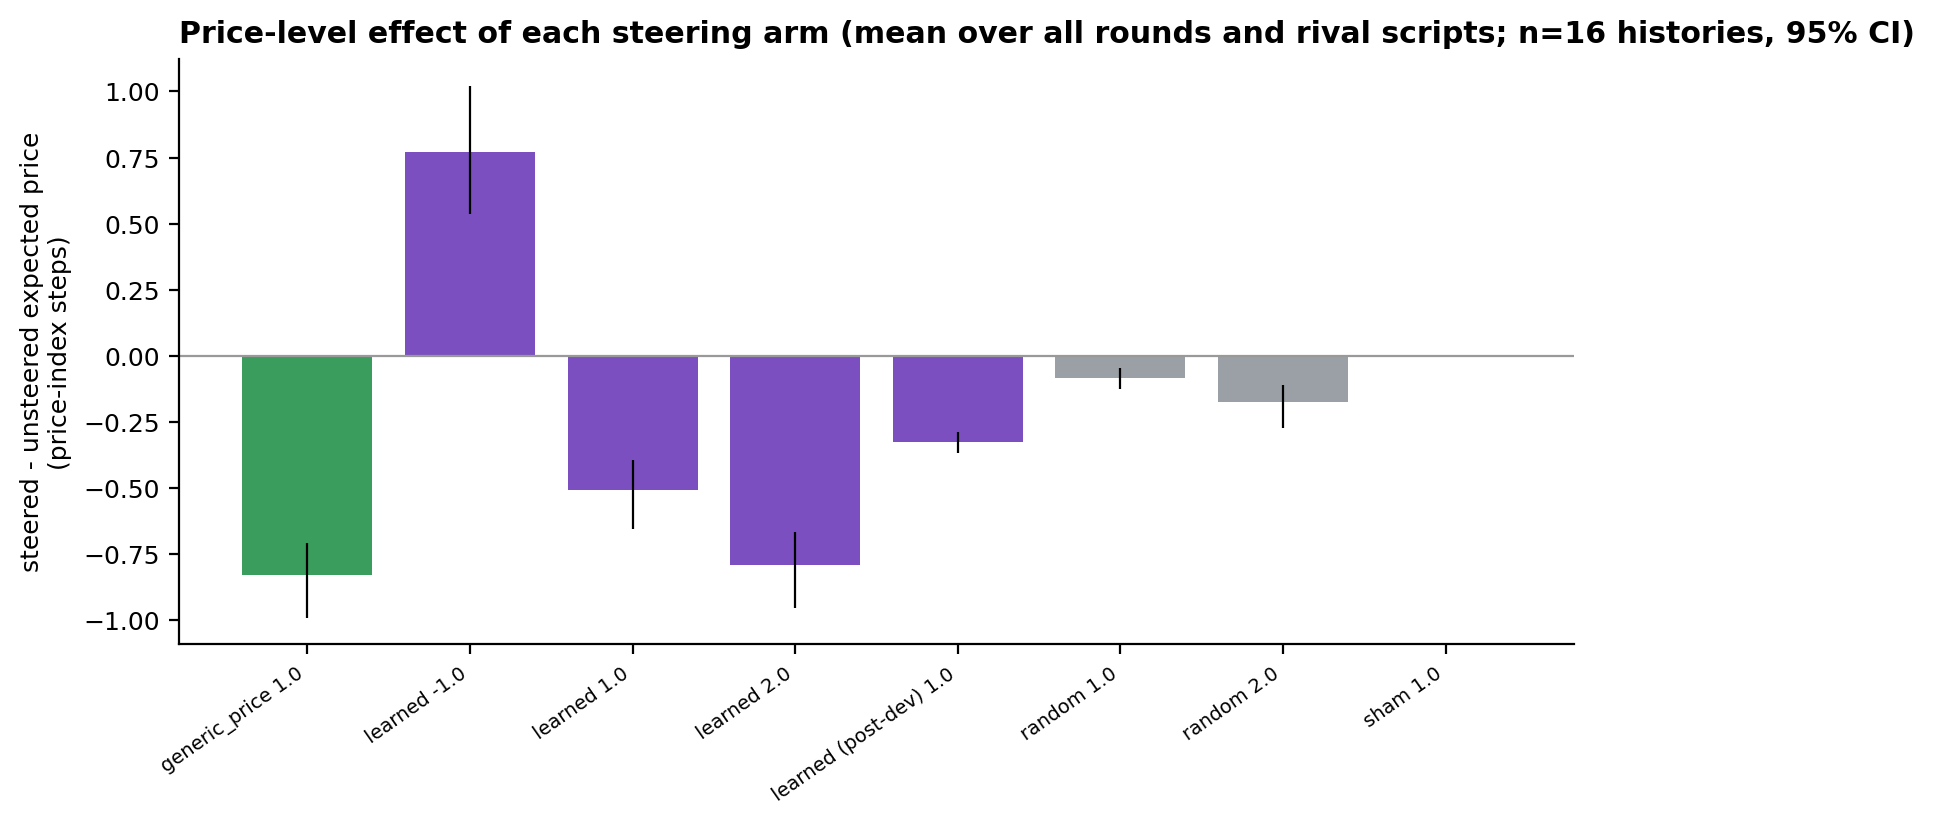
\includegraphics[width=0.58\textwidth]{figs/05_steering_vs_random.png}
\caption{Price-level effect of each steering arm, averaged over all rounds and rival scripts (16 histories, 95\% CI). The learned vector (purple) moves the price well beyond norm-matched random directions (grey) or the inert zero-vector sham.}
\label{fig:steervsrandom}
\end{figure}

This causal result does not establish that the located direction is specific to rival-price information. The vector's cosine similarity with the model's general high-versus-low price direction is 0.77--0.81, meaning a substantial part of its effect may be a shared route for price-level control rather than a feature reserved for processing the rival's price specifically; a norm-matched vector built from the irrelevant-number edits moves prices in the opposite direction, so not every direction at this site is inert, but specificity relative to the general price axis is not established.

The pre-registered follow-up on strategic deviation (1,656 confirmatory runs, 16 independent pre-play histories, 0 failed runs, every output strictly parsed) tested five hypotheses with Holm-corrected, cluster-bootstrap 95\% confidence intervals. Only the steering-specificity hypothesis was supported: at steering strength $+1$, the learned vector lowered price by 0.51 steps against 0.08 for norm-matched random directions (difference $-0.43$, 95\% CI $[-0.56,-0.32]$, Holm $p=0.002$). The model's immediate response to a one-off rival undercut was not distinguishable from zero ($-0.08$ steps, 95\% CI $[-0.25,0.09]$, Holm $p=0.81$); a delayed price fall did appear two to four rounds after an undercut (0.71 steps below the stable-rival control, consistent across all 16 histories), but an unexpected rival price \emph{increase} produced a fall of similar or larger size (Figure \ref{fig:deviation}), so this delayed response is better read as a reaction to any break in the rival's established pattern than as a punishment response specific to undercutting. A one-factor-at-a-time robustness batch (656 runs) found the high-price default itself (collusion index 0.73--0.95) stable across prompt templates, sampling temperature, and most economic settings, while the punishment-like and recovery effects were template-dependent and did not replicate consistently across settings.

\begin{figure}[H]
\centering
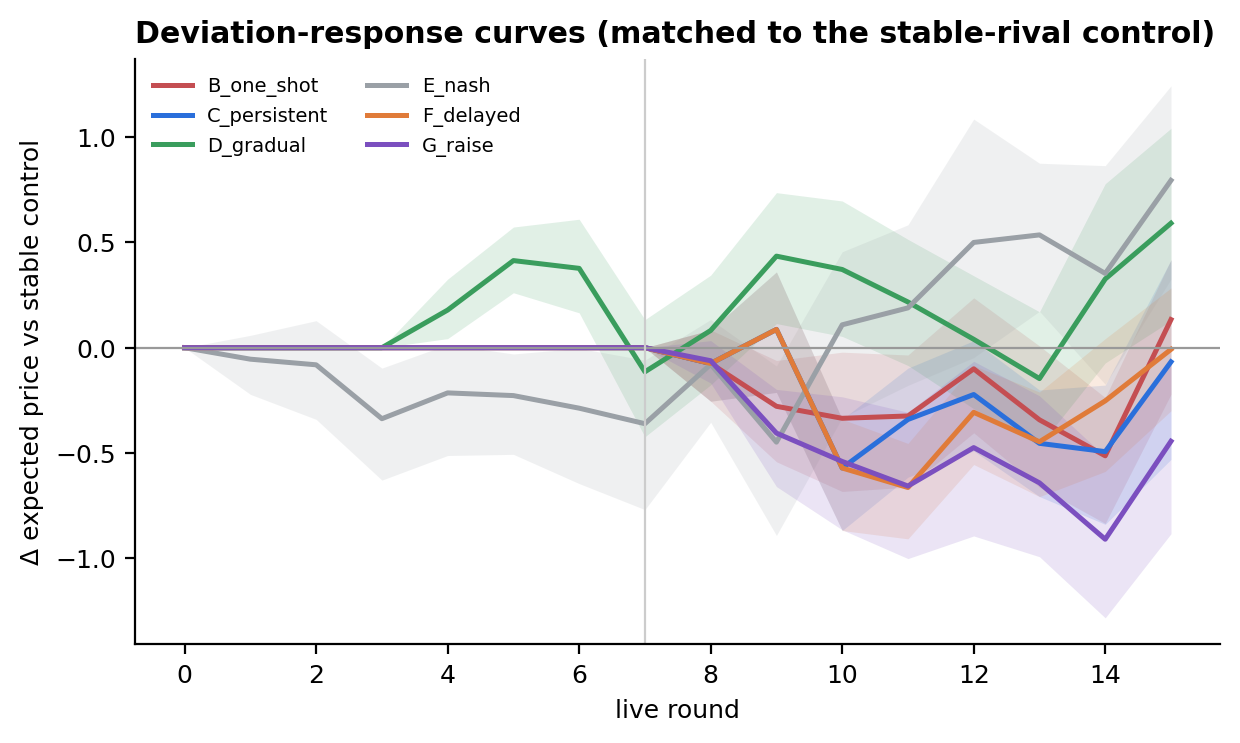
\includegraphics[width=0.6\textwidth]{figs/02_deviation_response.png}
\caption{Price response, relative to the stable-rival control, following each type of rival deviation (16 histories, shaded band = 95\% CI). The price fall following a rival price increase (G\_raise) is comparable to the fall following an undercut (B/C/F), consistent with a reaction to change in the rival's pattern rather than to undercutting specifically.}
\label{fig:deviation}
\end{figure}

Read together, these results support a causal link between the rival's displayed price and the model's output, and a located site at which that link can be intervened on, but do not support either of two stronger claims: that the mechanism is specific to rival-price information as opposed to price level in general, or that the model's pricing implements a recognizable punishment strategy. The dominant pattern across every batch (collusion index 0.73--0.95; see Figure \ref{fig:collusionindex}) is a persistent, largely rival-independent high-price default.

\begin{figure}[H]
\centering
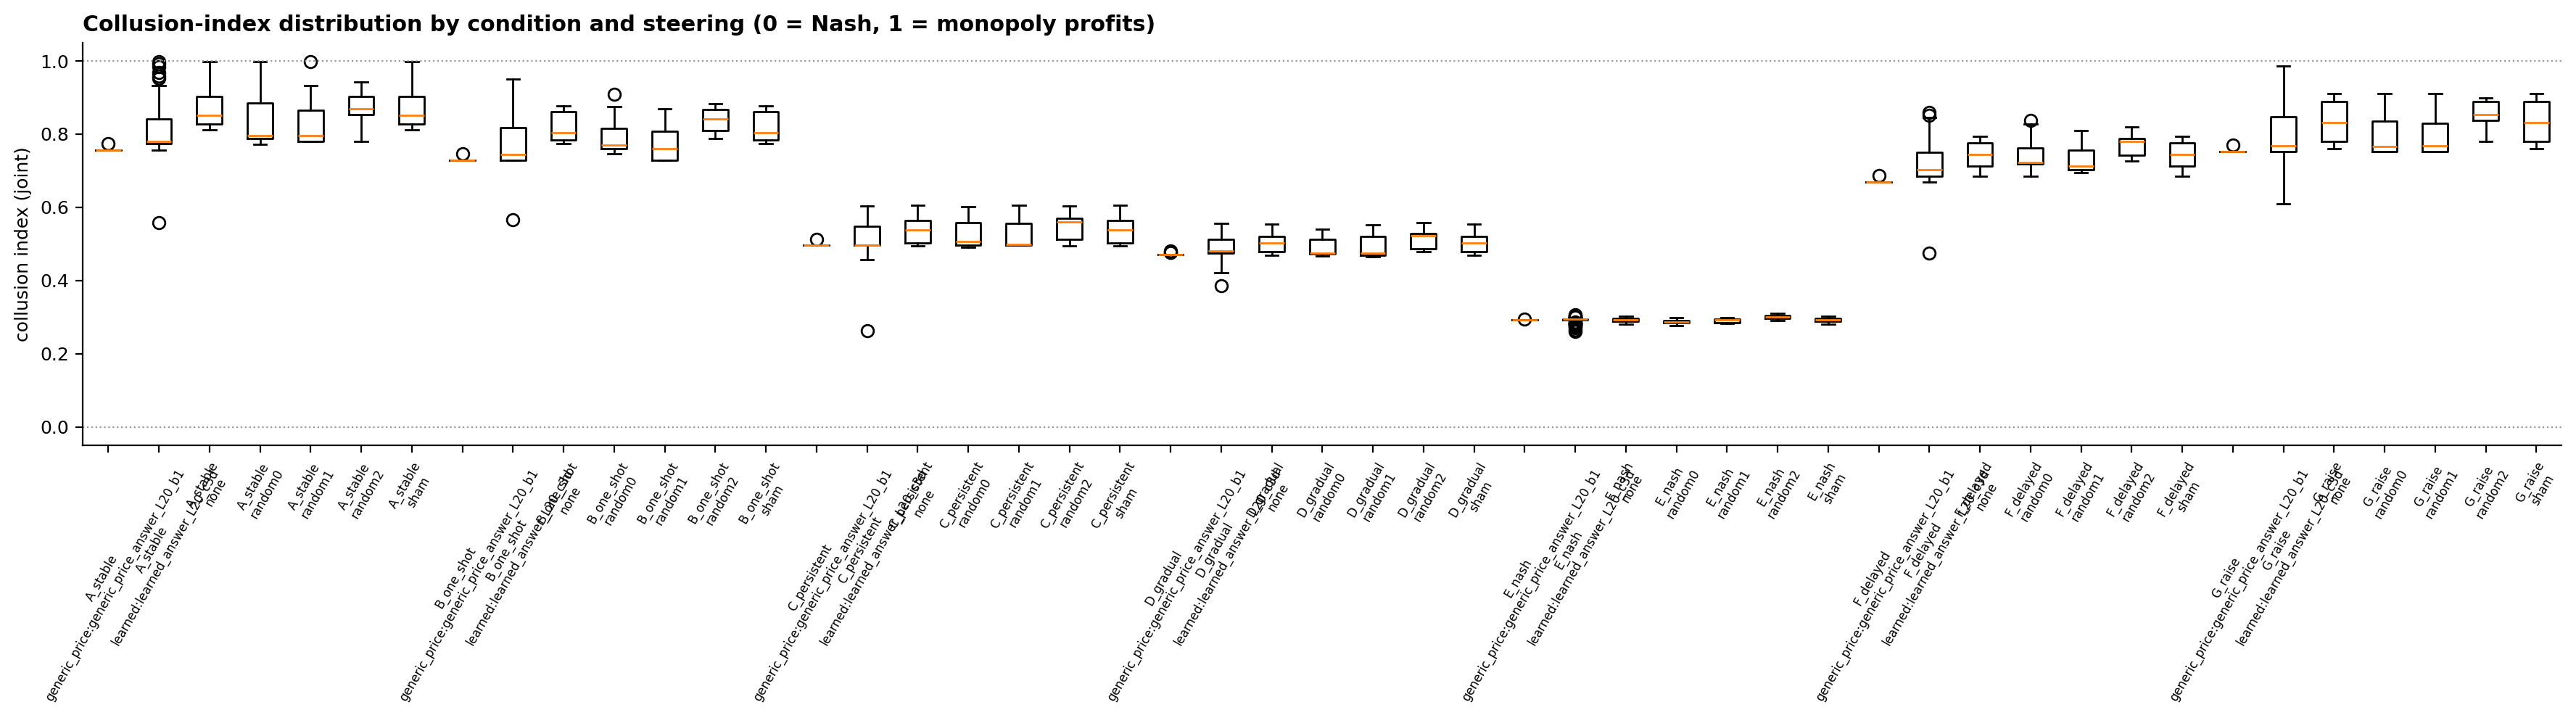
\includegraphics[width=0.8\textwidth]{figs/18_collusion_index.png}
\caption{Distribution of the collusion index (0 = Nash, 1 = monopoly profits) across rival conditions and steering arms in the confirmatory and robustness batches. The index remains supra-competitive in most conditions, consistent with a default rather than a rival-conditioned policy.}
\label{fig:collusionindex}
\end{figure}

\section{Further Observations (Hackathon-Track Experiments)}

Three additional, smaller experiments were run on the hackathon starter repository's environments, local inference only, no external API keys used. These are reported here as verified observations rather than full methods/results treatments; the pre-registered evidence standards, run logs, and complete analysis for each are documented in the project README.

\begin{itemize}[leftmargin=1.4em]
\item \textbf{Action-carrier visibility (Cournot market).} A three-condition ablation tested whether making a rival's exact past quantity visible, rather than hidden or coarsely rounded, increases market specialization. At 8 pairings per condition, the specialization measure (coefficient of variation) was 0.408 under the hidden baseline, 0.417 under the rounded condition, and 0.443 under the visible condition (Figure \ref{fig:cournotcv}); the three 95\% confidence intervals overlap substantially, and the rounded condition does not sit between the other two as the hypothesis would predict. We do not find support for an action-carrier channel at this scale; a larger-scale run intended to resolve the overlap was attempted twice on Modal and failed both times on a recurring infrastructure disconnect, which was not resolved within the sprint.

\item \textbf{Surveillance-awareness replication (double auction).} A positive-control run (communication enabled, no oversight) was required to clear the environment's own cartel-pricing detection threshold before testing whether stated surveillance changes pricing. Neither a 7B nor a 32B open model cleared this threshold across the tested round counts, so the oversight-awareness manipulation itself was not run. Independently of this, 22\% of the 32B model's messages contained price-coordination language that a pre-registered keyword list, carried over from an earlier experiment in a different environment, failed to flag.

\item \textbf{Mid-run model-identity swap.} In a repeated trust game, an incumbent agent was asked to judge, after the fact, whether its counterpart's underlying model had been silently swapped partway through. At five pairings per condition, a genuine swap (from a 0.5B to a 7B model) was correctly identified in 5 of 5 cases, with a measurable behavioral discontinuity (the swapped agent's commitment-breaking rate fell from 81\% to 25\% at the swap point). In a no-op condition with no real swap, the incumbent still answered "changed" in 3 of 5 cases at the same confidence level, indicating that the explicit judgment is not well calibrated at this sample size: it may be responding to any apparent inconsistency rather than to evidence of a real swap. A larger run (fifteen pairings per condition, including a cross-provider condition) was in progress at the time of writing and is not included here.
\end{itemize}

\begin{figure}[H]
\centering
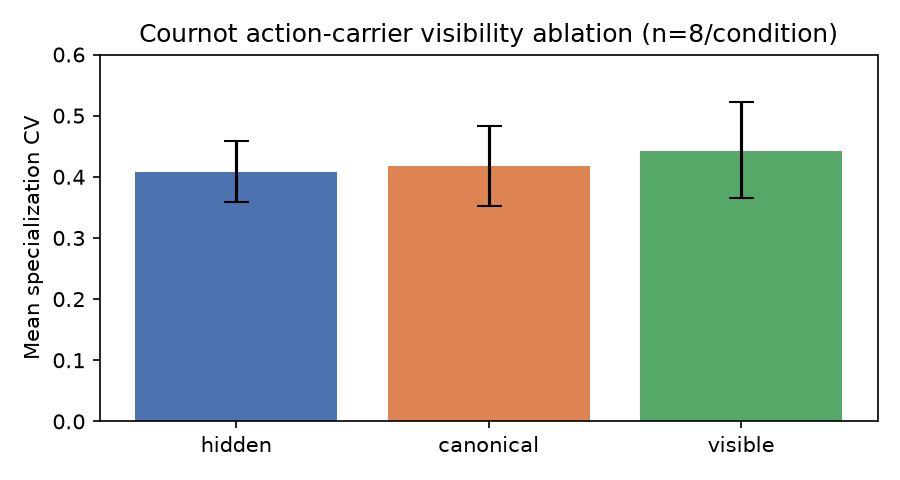
\includegraphics[width=0.5\textwidth]{figs/cournot_cv.png}
\caption{Mean specialization (coefficient of variation) across the three Cournot visibility conditions, 8 pairings per condition, 95\% CI.}
\label{fig:cournotcv}
\end{figure}

\section{Discussion and Limitations}

Both lines of work reported in detail point to a similar practical conclusion from different directions: the tabular and LLM pricing agents studied here do not behave as if they are reasoning about the rival's strategy and responding to it in an economically grounded way. In the Bertrand market, the cheapest intervention is not a smarter detector or a larger number of competitors but a single fixed agent that refuses to collude. In the mechanistic study, the model's dominant behavior is a fixed high-price default that is largely insensitive to what the rival actually does, including to being undercut, even though a located activation site can be shown to carry \emph{some} causal influence of the rival's price on the model's output. Neither result should be read as evidence that the model understands or intends coordination; both are consistent with the price level being a default learned or prompted behavior that external interventions can suppress without addressing.

\textbf{Limitations.} The mechanistic results concern a single open-weight model family (Qwen2.5, principally the 7B variant) and scripted, non-learning rivals; nothing in this report tests two LLM agents conditioning on each other over repeated play, which would be needed before any claim about coordination between two LLMs specifically could be made. The steering vector's specificity relative to a general price-level direction is not established, and this is reported as an open limitation rather than resolved. Sample sizes throughout are small relative to what a fully powered study would require (16 independent histories in the confirmatory mechanistic batch, 5 and 8 pairings per condition in the two smallest hackathon-track experiments); confidence intervals are reported wherever available so that readers can judge this directly rather than relying on point estimates. The two hackathon-track results reported as negative (the visibility ablation and the surveillance-awareness positive control) are negative at the scale we were able to run, not confirmed negatives; in both cases a larger run that might have resolved the ambiguity was attempted and did not complete, for reasons documented in the repository.

\textbf{Future work.} A larger run of the Bertrand/LLM validation pass with more seeds and additional model families would clarify whether the exploration-time and replacement findings generalize beyond \texttt{qwen2.5:7b-instruct}. On the mechanistic side, extending the probing and steering pipeline to the 14B and 32B models (which, unlike 7B, respond to a rival price change in the direction the one-round best response predicts) and to genuine two-LLM self-play would test whether the located mechanism generalizes and whether it supports any claim about coordination rather than a shared default.

\section{Conclusion}

We report two detailed experimental threads on tacit collusion in pricing agents. The first shows that a repeated Bertrand market's collusive equilibrium, reproduced for both tabular Q-learning and an LLM agent, is disrupted most cheaply by introducing one fixed, non-cooperative agent, not by adding competitors or restricting the strategy space. The second shows that an LLM pricing agent's response to a rival's price has a locatable, causally intervenable substrate in its activations, but that this mechanism is not specific to the rival's price as distinct from price level in general, and does not implement a punishment-like response to undercutting under a pre-registered confirmatory test. Three further, smaller hackathon-track observations are summarized in Section 5 at the level of verified results, with full methodology and raw outputs available in the project repository.

\section*{Limitations and Dual-Use / Ethical Considerations}
\textbf{What this report does and does not establish.} We establish that (a) in a specific repeated Bertrand environment, introducing one fixed non-cooperative agent is a cheaper disruption to tacit collusion than adding competitors, for both tabular Q-learning and one LLM; and (b) in a specific pricing environment, one LLM's price is causally influenced by a rival's displayed price through a locatable activation site, but that this mechanism is not shown to be specific to rival-price information, does not implement a punishment-like response to undercutting, and has not been tested in genuine two-LLM self-play. We do not establish that these findings generalize to other models, environments, market structures, or real deployed pricing systems; we do not establish that any model studied here "intends" to collude, only that its behavior is supra-competitive and, in the mechanistic study, partly steerable. The hackathon-track observations in Section 5 are reported at small sample sizes and should not be treated as settled negative or positive results.

\textbf{Dual-use considerations.} The disruption finding (one fixed competitive agent breaks collusion cheaply) is intended as a defensive result: it identifies a low-cost way to suppress tacit collusion in a deployed multi-agent pricing system. The same finding could in principle inform an adversary trying to predict how few "honest" participants a market needs before a collusive equilibrium collapses, but this is a direct restatement of findings already published in the cited prior work (Calvano et al., 2020) rather than a new capability. The mechanistic steering result demonstrates that a pricing LLM's output can be pushed lower (toward more competitive pricing) with an activation-space intervention; the same intervention, applied in the opposite direction, would push prices higher, which is a capability for inducing rather than suppressing collusive-looking pricing. We report this because understanding that such an intervention exists, and the extent to which it is non-specific (Section 4.2), is necessary for anyone building a monitoring or control system around pricing LLMs; we are not aware of a way to describe the causal finding without describing the direction in which it generalizes. No part of this work was used against a real market or deployed pricing system, and all experiments used synthetic environments, open-weight models run locally or on rented compute, and no production data.

\section*{Code and Data}
\begin{itemize}[leftmargin=1.4em]
\item Code repository: \url{https://github.com/Peddinti-Sriram-Bharadwaj/Collusion}. The repository README documents every experiment referenced in this report, including those summarized briefly in Section 5, with full hypothesis/setup/result/analysis write-ups, run logs, and figures not reproduced here.
\item The mechanistic-analysis experiments are on the \texttt{gagana/latent-manifold-steering} branch of the same repository (run registry, raw results, and figure source files under \texttt{research/}).
\end{itemize}

\section*{References}
\begin{enumerate}[leftmargin=1.6em]
\item Calvano, Calzolari, Denicol\`o, Pastorello (2020). Artificial Intelligence, Algorithmic Pricing, and Collusion. \emph{American Economic Review}.
\item Fish, Gonczarowski, Shorrer (2024). Algorithmic Collusion by Large Language Models. arXiv:2404.00806.
\item Agrawal et al.\ (2025). Evaluating LLM Agent Collusion in Double Auctions. arXiv:2507.01413.
\item Lin et al.\ (2024). Strategic Collusion of LLM Agents: Market Division in Multi-Commodity Competitions. arXiv:2410.00031.
\item Shi et al.\ (2026). When Agents Lie: Premeditation, Persistence, and Exploitation in Repeated Games. arXiv:2607.05132.
\item Motwani et al.\ (2024). Secret Collusion among AI Agents. arXiv:2402.07510.
\item Tailor (2025). Audit the Whisper: Detecting Steganographic Collusion in Multi-Agent LLMs. arXiv:2510.04303.
\item Kale et al.\ (2025). [Surveillance-awareness source paper, double-auction environment.]
\item Oversight is Not Compliance. ICML 2026.
\end{enumerate}

\section*{Appendix: Glossary of Terms}

\subsection*{Market and economics concepts}
\textbf{Tacit collusion.} Prices or outcomes that look coordinated without any agent ever communicating an agreement, as opposed to an explicit cartel.

\textbf{Supra-competitive pricing.} A price above what a competitive market would produce.

\textbf{Nash price / Nash equilibrium.} The price each seller would charge under pure, uncoordinated self-interest; the competitive benchmark.

\textbf{Monopoly price.} The price a single firm would charge if it owned the entire market; the benchmark for full collusion.

\textbf{Collusion index ($\Delta$).} $\Delta = (\text{actual profit} - \text{Nash profit})/(\text{monopoly profit} - \text{Nash profit})$. 0 = competitive, 1 = fully collusive.

\textbf{Marginal cost.} The cost of producing one additional unit.

\textbf{Market share.} The fraction of total sales a firm captures.

\textbf{Logit demand.} A demand rule where customers split smoothly between sellers by price rather than all switching at once to the cheapest option.

\textbf{Double auction.} A market where buyers and sellers each submit offers, with trades occurring when an offer and ask match.

\subsection*{Environments used in this project}
\textbf{Bertrand pricing game.} Firms simultaneously set a price each round from a fixed grid; demand splits by the logit rule. The main environment for the tracks in Section 4.1.

\textbf{Cournot game.} Firms set quantities rather than prices; price falls out of total quantity produced. Used in the visibility-ablation lane (Section 5).

\textbf{Market division / specialization.} In the Cournot setting, firms tacitly retreating into one product each rather than competing on both; measured by the coefficient of variation (CV) of a firm's own quantities across products.

\textbf{Liar's Bar.} A multiplayer bluffing game (players challenge each other's claims) used to test whether a trusted agent can expose willingness to collude.

\textbf{Diner's Dilemma.} A repeated two-player trust game (private plan, public announcement, final action) used to measure commitment-breaking and swap detection.

\subsection*{Machine learning and interpretability concepts}
\textbf{Tabular Q-learning.} A non-LLM learning method that keeps a table of expected reward per situation/action and updates it from experience.

\textbf{Exploration vs.\ exploitation.} The trade-off between trying new actions and sticking with ones known to work.

\textbf{Activations / hidden states.} An LLM's internal numerical representation at each layer while processing a prompt.

\textbf{Linear probe.} A small auxiliary model trained to decode a specific piece of information directly from an LLM's activations.

\textbf{Activation patching.} Swapping activations between two matched prompts at a chosen layer/position to test whether that site causally carries a given effect.

\textbf{Steering vector.} A direction added into a model's activations at a chosen site to push its output in a predictable direction.

\textbf{Specificity (steering).} Whether a steering vector's effect is tied to the specific feature it was built from, or rides along a more general direction the model already has.

\subsection*{Statistics}
\textbf{Confidence interval (CI).} A range likely to contain the true value given the collected data; overlapping CIs between two groups generally mean no confidently distinguishable difference.

\textbf{p-value / Holm correction.} A p-value measures how surprising a result would be under no real effect; the Holm correction tightens the significance threshold when testing multiple hypotheses at once.

\textbf{Pre-registration.} Fixing hypotheses and success criteria before running the main batch of an experiment, to prevent post-hoc reinterpretation of results.

\textbf{Spearman correlation ($\rho$).} A $-1$ to $1$ measure of whether two variables move together in rank order.

\textbf{Coefficient of variation (CV).} A measure of spread relative to the mean; used as the specialization measure in the Cournot lane.

\subsection*{AI-safety vocabulary}
\textbf{Distributional risk.} Risk arising from how many independently "reasonable" AI systems interact in aggregate, rather than from any single system's misbehavior.

\textbf{AI control / oversight.} Techniques for constraining an AI system's behavior without relying solely on trusting its stated intentions, e.g.\ a trusted system monitoring or editing an untrusted one.

\textbf{Surveillance / evaluation awareness.} Whether an agent's behavior changes specifically because it knows it is being watched or evaluated.

\textbf{Sandbagging.} An AI system deliberately underperforming during evaluation to appear less capable than it is.

\textbf{Steganographic / covert-channel collusion.} Coordination carried out through disguised signals (paraphrased language, timing, actions) that evade a straightforward monitor.

\textbf{Action-carrier / side channel.} Coordination conveyed through an action rather than an explicit message, which a message-only monitor would miss.

\textbf{Positive / negative control.} A condition expected to clearly show the effect under study (confirms the setup works) or clearly not show it (confirms the measurement isn't pure noise), respectively.

\textbf{Decision gate.} A rule fixed in advance for when to stop a line of experiments rather than continue once a precondition has failed.

\section*{LLM Usage Statement}
Claude (Anthropic) was used during this project to draft experiment code, debug infrastructure (Modal, vLLM, Ollama), run and monitor background experiments, and draft this report from the underlying experiment logs, analysis scripts, and progress notes supplied by the authors. Numerical results reported here are taken from those underlying outputs rather than generated by the drafting process; the authors reviewed and are responsible for the final claims.

\end{document}
